\documentclass[pdf,mpa]{prosper}

\FontText{\usefont{T1}{phv}{m}{n}\fontsize{16.4pt}{16pt}%
  \selectfont}{%
  \usefont{T1}{phv}{m}{n}\fontsize{16.4pt}{16pt}\selectfont}

\NewSlideStyle[13.5cm]{t}{5.5,3.5}{}



\usepackage{german}
\usepackage{amsfonts,amsmath}
\usepackage{url}
\usepackage[dvips]{graphicx}
\usepackage[latin1]{inputenc}

\usepackage[all,cmtip,ps,line,dvips]{xy}


\raggedright

% \newcommand{\kopf}[1]{{\tiny\tt #1} \par}
\newcommand{\kopf}[1]{}
\newcommand{\titel}[1]{\underline{\Large {#1}}}

\newcommand{\CF}{\mathsf{CF}}
\newcommand{\REG}{\mathsf{REG}}
\newcommand{\SL}{\mathsf{SL}}
\newcommand{\ZZ}{\mathbb{Z}}
\newcommand{\NN}{\mathbb{N}}

\newcommand{\FC}{\mathsf{FC}}
\newcommand{\RC}{\mathsf{RC}}
\newcommand{\RRC}{\mathsf{RRC}}
\newcommand{\OVL}{\mathsf{OVL}}
\newcommand{\Nf}{\mathsf{Nf}}


\title{
  The Leipzig \emph{autotool} E-Learning/E-Testing system
}
\author{ 
  Mirko Rahn, Univ. Karlsruhe \\
  Alf Richter, Univ. Leipzig \\
  \emph{Johannes Waldmann}, HTWK Leipzig
}  
\slideCaption{Math Tutoring Symposium, Heerlen 08}


\begin{document}
\maketitle


\begin{slide}{Example: Graph Colouring (Instance)}

\begin{minipage}{0.4\textwidth}
\includegraphics[width=7cm]{536970904.Dot.eps}
\end{minipage}%
\begin{minipage}{0.5\textwidth}
\begin{small}
\begin{verbatim}
Give a conflict-free node colouring of
Graph { knoten = mkSet [ 1 , 2 , 3 , 4 , 5 , 6 , 7 , 8 , 9 , 10 ]
  , kanten = mkSet [ kante 1 6 , kante 1 7 , kante 1 9 , kante 2 5
     , kante 2 7 , kante 2 8 , kante 2 9 , kante 3 6 , kante 3 7
     , kante 3 8 , kante 3 9 , kante 4 5 , kante 4 6 , kante 4 7
     , kante 5 6 , kante 5 10 , kante 6 7 , kante 6 8 , kante 6 10
     , kante 8 9 , kante 8 10 , kante 9 10 
     ] 
  }
with at most 3 different colours.
\end{verbatim}
\end{small}  
\end{minipage}

\end{slide}

\begin{slide}{Example: Graph Colouring (Solution)}
Input
\begin{small}
\begin{verbatim}
listToFM [ ( 1 , C ) , ( 2 , C ) , ( 3 , B ) , ( 4 , B ) , ( 5 , B )
    , ( 6 , A ) , ( 7 , A ) , ( 8 , C ) , ( 9 , C ) , ( 10 , C ) 
\end{verbatim}
\end{small}
Grading:
\begin{small}
\begin{verbatim}
is the set
    nodes of graph =
    mkSet [ 1 , 2 , 3 , 4 , 5 , 6 , 7 , 8 , 9 , 10 ]
a subset of the set
    coloured nodes = mkSet [ 1 , 2 , 3 , 4 , 5 , 6 , 7 , 8 , 9 , 10 ]
? Yes.
These edges connect nodes of equal colour:
    [ kante 1 9 , kante 2 8 , kante 2 9 , kante 4 5 , kante 6 7
    , kante 8 9 , kante 8 10 , kante 9 10 ]
\end{verbatim}
\end{small}

\end{slide}

\begin{slide}{Typical \autotool\ Use Case}

Problem (Ex: COL)
\begin{itemize}\itemsep 2pt
\item Instance:  graph $G$, number $k$
\item Solution: a $k$-colouring of $G$
\end{itemize}

workflow \autotool\ :
\begin{itemize}\itemsep 2pt
\item \emph{tutor} configures \emph{generator} 
\item \emph{student} starts working:  \\
  \autotool\ generates problem instance
\item student types in candidate solution
\item \autotool\ verifies candidate, \\
  reports back (verbose, immediately)
\end{itemize}

\end{slide}




\begin{slide}{Example: Graph Colouring (Configuration)}

the tutor did choose this:
\begin{itemize}
\item semantics:

problem type: \verb|Col-Quiz| and parameters for generator
\begin{verbatim}
Config { nodes = 10 , edges = 30 , chi = 3 }
\end{verbatim}
\item bookkeeping:

school, lecture, exercise, time span, rating (level)
\end{itemize}

\end{slide}

\begin{slide}{Problem levels}

problems are marked as
\begin{itemize}
\item Demo (``too easy'', for illustration)
\item Mandatory (must submit at least one correct solution before deadline,
  any number of attempts allowed)
\item Optional (``too hard'', prize questions etc.)
\end{itemize}

even after deadline, student can
\begin{itemize}
\item
  work on problems (will be graded, but not counted)
\item
  review previous graded answer
\end{itemize}
useful e.g. when preparing for exams

\end{slide}


\begin{slide}
\titel{Themen}

\begin{itemize}
\item
  formale Sprachen:

  Grammatiken (alle Chomsky-Typen), regul�re Ausdr�cke
\item
  Automaten/Berechnungsmodelle:

  endlich (Wort, Baum), Keller, Turing, Registermaschine,
  (primitiv) rekursive Funktionen
\item
  Graphen: 

  Parameter, F�rbungen, Wege
\item
  diskrete Mathematik und Logik:

  Aussagenlogik, Zahlendarstellungen
\item
  Datenstrukturen:

  (balancierte) Suchb�ume
\end{itemize}


\end{slide}

\begin{slide}{\autotool\ as a verifier}

\begin{itemize}
\item
  ideally, problem is in NP (e.g. COL):
  \begin{itemize}
  \item
    student has to guess (N)
  \item
    \autotool\ has to check (P)
  \end{itemize}
\item
  sometimes solutiones are a bit longer (PCP)
\item
  or verification takes a bit longer 
  (equivalence of regular expressions)
\item
  sometimes verification is impossible,

  then replaced by testing (equivalence of CFG)
\end{itemize}

lots of opportunities to discuss with students
about decidability and complexity
\end{slide}


% \begin{slide}{Wichtige Datentypen}

(f�r Automaten und Sprachen)
\begin{itemize}
\item endlicher Automat, Kellerautomat
\item Grammatik
\item regul�rer Ausdruck
\end{itemize}

Repr�sentation m�glichst nahe an der mathematischen Wahrheit,

statt Tupel benutze Strukturen mit benannten Komponenten,

geschweifte Klammern sind daf�r reserviert,
deswegen Mengen als \verb|mkSet [ 1, 2, 3 ]|

\end{slide}


% \begin{slide}{Endliche Automaten}

\begin{small}
\begin{verbatim}
NFA { alphabet = mkSet "ab" , states = mkSet [ 1, 2, 3 ]
    , starts = mkSet [ 2 ] , finals = mkSet [ 2 ]
    , trans = collect 
          [ ( 1, 'a', 2 ), ( 2, 'a', 1 )
          , ( 2, 'a', 3 ), ( 2, 'b', 3 ), ( 3, 'b', 2 )
          ]
    }
\end{verbatim}
\end{small}  

Eigenschaften 
(f�r Test der Einsendungen und ggf. Konfiguration der Generatoren)

\begin{verbatim}
   Min_Size Int | Max_Size Int 
 | Alphabet ( Set c )
 | Deterministic | Minimal | Complete | Reduced 
\end{verbatim}
  
\end{slide}

% \begin{slide}{Regul�re Ausdr�cke}

\begin{verbatim}
((ba)^* + (bb)^*)^* + (ab)^*
\end{verbatim}

Definition:
\begin{itemize}
\item
  atomar: Buchstabe oder Name (\verb|Sigma, All|)
\item 
  zusammengesetzt mit Operationen:

  Verkettung (\verb|.|), Vereinigung \verb|+|, 
  Durchschnitt \verb|&|, Differenz \verb|-|,
  symmetrische Differenz \verb|<>|,
  Shuffle \verb|$|, Quotienten \verb|\,/|,
  Potenzen \verb|^int, ^*, ^+|
\end{itemize}

Eigenschaften:
\begin{verbatim}
   Min_Size Int | Max_Size Int | Alphabet ( Set c )
  | Simple -- nur Plus, Mal, Stern
  | Extended -- alles
\end{verbatim}


\end{slide}

% \begin{slide}{Grammatiken}

\begin{small}
\begin{verbatim}
Grammatik { terminale = mkSet "01"
          , variablen = mkSet "ST"
	  , start = 'S'
	  , regeln = mkSet [ ( "S", "" ), ( "S", "T0S" ), ( "T", "11" ) ]
	  }
\end{verbatim}
\end{small}  

Eigenschaften:
\begin{itemize}
\item monoton, kontextsensitiv, kontextfrei, linear, rechts/links-linear, 
\item f�r CFG: epsilon-frei, ketten-frei, Chomsky-normal, Greibach-normal
\item eindeutig (nat�rlich nur Test)
\end{itemize}


\end{slide}

% \begin{slide}{Find a small context-free grammar}

\newcommand{\reverse}{\mathop{\textrm{reverse}}}

for $L = \Sigma^* \setminus \{w w \mid  w \in\Sigma^* \}$
where $\Sigma=\{0,1\}$.

solution plan
\begin{itemize}
\item $L \to AB, L \to BA$ (start)
\item $A \to 0, A \to SAS$ (0 in the middle)
\item $B \to 1, B \to SBS$ (1 in the middle)
\item $S \to 0,S \to 1$ (any letter)
\end{itemize}
which words are missing? (easy)

how to create them with \emph{two} (not three) additional rules?

\end{slide}


\begin{slide}{Einsatz in Lehrveranstaltungen}

\begin{itemize}
\item
  Automaten und Sprachen,
  Berechenbarkeit und Komplexit�t
  (Uni Leipzig ab 2001, Uni Halle ab 2006)
\item
  Automaten und Sprachen im Compilerbau (HTWK Leipzig, ab 2003)
\item
  Datenstrukturen, diskrete Mathematik in Grundlagen der Informatik (Nebenfach)
  (HTWK L ab 2003)
\item
  Datenstrukturen, disk. Math. in Grundl. Inf. (Nebenfach)
  (Uni Karlsruhe ab 2005, Uni Halle ab 2006)
\end{itemize}


\end{slide}

\begin{slide}{Erfahrungen}

\begin{itemize}
\item
  \autotool\ zur Unterst�tzung des �bungsbetriebes.

  etwa die H�lfte der Aufgaben mit \autotool\ korrigieren
  \dots die andere H�lfte: schriftliche (Beweis-)Aufgaben
\item
  wird von Studenten gut angenommen, 

  sind erfreut �ber sofortige, ausf�hrliche Antwort.
\item
  Highscore-Wertung (mit Preisen) schafft zus�tzlichen Anreiz
\item
\end{itemize}

\end{slide}


\begin{slide}{Installation, Nutzung}

\emph{separate Installation}:
\begin{itemize}
\item
  halbwegs schnellen Rechner mit GNU/Linux, Apache Webserver,
  GHC-Compiler, MySQL-Datenbankserver 
\item
  daf�r Administrator, der System und Datenbank einrichtet
  und im Betrieb bei Bedarf Patches einspielt und kompiliert
\end{itemize}

\emph{zentrale Installation}: Benutzung eines gemeinsamen 
\autotool-Servers (@ HTWK) durch mehrere Einrichtungen 
(HTWK, Uni Leipzig, Uni Halle)


\end{slide}

\begin{slide}{Bestandteile des \autotool}

\begin{itemize}
\item
  Semantik-Bibliothek

  (Automaten, Grammatiken, Graphen, \dots)
\item
  Generator-Programme
\item
  Korrektur-Programme
\item
  Datenbank 

  Konfiguration der Generatoren,  Aufgaben

  erreichte Punkte
\item
  Web-Schnittstelle

  f�r Studenten, f�r Tutoren
\end{itemize}

\end{slide}

\begin{slide}{\autotool\ intern}

\parskip 5pt 

implementiert in Haskell 
(purely functional, strictly typed, polymorphic, lazy)

von Waldmann, Rahn, Richter seit ca. 2001

einige Teile waren Belegarbeiten f�r Vorlesung
Funktionale Programmierung (Gerber)

Umfang:
\begin{itemize}
\item
  Bibliothek 
  (allg. Datenstrukturen und endliche Automaten): 
  300 Module, 15 kLOC; 
\item
  Tool: 600 Module, 45 kLOC
\end{itemize}
(10 Zeilen pro Arbeitstag (Fred Brooks, 1972) $\to$ \dots)

\end{slide}

\begin{slide}{Weiterentwicklung}

\begin{itemize}
\item
  derzeit Waldmann (Leipzig) und Rahn (Karlsruhe)
  nach \glqq Eigenbedarf\grqq
\item
  Bibliothek nachgenutzt f�r Matchbox (180 Module, 15 kLOC)
  (findet Beweise f�r Termination von Wort- und Termersetzungssystemen)
\end{itemize}

f�r systematische Weiterentwicklung und Aufr�um-Arbeiten
(Oberfl�che, Dokumentation):
ben�tigen  HiWis oder Diplomanden 
mit Kenntnissen in Funktionaler Programmierung

(Vorlesung ab SS06 an HTWK)

\end{slide}


\begin{slide}{Informatik I (als Nebenfach)}

\begin{itemize}
\item
  Einf�hrung Algorithmen, Sortieren:

  \emph{Sortiernetze}
\item
  Komplexit�t (Suchprobleme): 

  \emph{COL} (NP), \emph{Lunar Lockout} (PSPACE),\emph{PCP} (RE)
\item
  Programmierung: 

  \emph{Collatz(/Inverse)}
\item
  Datenstrukturen: 
  
  \emph{Suchb�ume (Einf�gen/L�schen)}
\end{itemize}

\end{slide}

\begin{slide}{Sorting Networks}


Find a sorting network for 5 inputs \\
with less than 10 comparator circuits


\begin{small}
\begin{verbatim}
mkNetz [ ( 1 , 4 ) , ( 3 , 4 ) , ( 2 , 3 ) , ( 1 , 2 ) , ( 3 , 5 ) ]
\end{verbatim}
\end{small}


\begin{minipage}{0.4\textwidth}
\begin{small}
\begin{verbatim}
This input
is not handled correctly:
[ 5 , 1 , 2 , 3 , 4 ]
The output
of the network is:
[ 1 , 3 , 2 , 5 , 4 ]
\end{verbatim}
\end{small}
\end{minipage}%
\begin{minipage}{0.5\textwidth}
\begin{small}
\begin{verbatim}
---------------------4--o--4---
                        v      
---3--o--5--o--5--------v------
      v     v           v      
------v--2--o--2--o--2--o--2---
      v           v            
------v--------1--o--1--o--3---
      v                 v      
---5--o--3-----------3--o--1---
\end{verbatim}
\end{small}
\end{minipage}

discuss: specification, correctness, lower bounds


\end{slide}

\begin{slide}{Search problem: Lunar Lockout}

\begin{minipage}{0.6\textwidth}
Cars at A,B,C,D,E; task: move E to e.
Car stops only when hitting other car.
\end{minipage}\quad
\begin{minipage}{0.3\textwidth}
\begin{verbatim}
. D . . . 
. . . . C 
B e . . . 
. . . . . 
. . E . . 
. . . . A 
\end{verbatim}
\end{minipage}

Solution
\begin{verbatim}
 [ ( "A" , N ) , ("A", W), ("A", N)
, ("C", W), ( "E" , N ), ("E", W) ] 
\end{verbatim}
discuss: configuration, number of configurations, bound
\end{slide}

\begin{slide}{Suchproblem: PCP}

L�sen Sie diese Instanz des Postschen Korrespondenz-Problems:
\begin{small}
\begin{verbatim}
 PCP [ ( "aa" , "ba" ) , ( "ab" , "a" ) , ( "c" , "a" )
     , ( "bac" , "accbac" ) ]
\end{verbatim}
  
\begin{verbatim}
gelesen: [ 2 , 1 , 2 , 4 ]

Aus Ihrer Folge entstehen die Zeichenketten:
abaaabbac
abaaaccbac

Die eine mu� ein Pr�fix der anderen sein,
nach L�schen des gemeinsamen Pr�fixes  "abaaa"
entstehen jedoch die Reste  ( "bbac" , "ccbac" )
\end{verbatim}
\end{small}
\end{slide}



\begin{slide}{Introduction to CS (minor subject) II}

\begin{itemize}
\item
  propositional logic: \emph{SAT, boolean functions}
\item
  number systems

  \emph{change of basis, floating point approximations}
\item
  codes: \emph{Hamming-distance}
\item
  compression: \emph{Huffman, Lempel-Zhiv}
\item
  cryptography

  \emph{gcd (extended), RSA}
\end{itemize}

\end{slide}


\begin{slide}{Aussagenlogik}

\begin{itemize}
\item
Finden Sie eine erf�llende Belegung f�r die Formel
$(p\wedge q\wedge \neg t)\vee(p \wedge r\wedge s)
\vee(p\wedge s\wedge t)\vee(p\wedge s\wedge r)
\vee(p \wedge t\wedge\neg s)\vee(q\wedge t\wegde \neg r)\vee \dots$

\item
Gesucht ist ein aussagenlogischer Ausdruck,
der �quivalent ist zu:
\begin{verbatim}
    ((y == ! z) || x && x) || y
\end{verbatim}
und nur diese Operatoren enth�lt:
\begin{verbatim}
    mkSet [ <= , false ]
\end{verbatim}
\end{itemize}

Diskussion:
Erf�llbarkeit, Entscheidbarkeit, Komplexit�t,
Boolesche Basisfunktionen

\end{slide}
%%% Local Variables: 
%%% mode: latex
%%% TeX-master: t
%%% End: 

\begin{slide}{Number systems}

\begin{itemize}
\item
  Convert
\begin{verbatim}
Zahl { basis = 3
  , ziffern = [1,0,1,0,0,1,1,0,0,1,2,1,0]
  }
\end{verbatim}
  to basis 5
\item
Among floating point numbers with
\begin{verbatim}
Config  { basis = 2 
  , max_stellen_mantisse = 3 
  , max_stellen_exponent = 3 }
\end{verbatim}
find the best approximation to 4 / 7.



\end{itemize}

\end{slide}
%%% Local Variables: 
%%% mode: latex
%%% TeX-master: t
%%% End: 

\begin{slide}{Codes: Hamming-distance}

Find a code (as set of words over L,R) with
\begin{verbatim}
Config { width = ( Fixed , 4 ) 
    , size = ( Atleast , 5 )
    , distance = ( Atleast , 2 ) 
    , optimize = Size }
\end{verbatim}
\bigskip
solution
\begin{verbatim}
[ [L,R,R,L], [R,L,L,R], [L,L,L,L]
, [R,R,R,R], [L,L,R,R] ]
\end{verbatim}
discuss: error detection, error correction,
triangle inequality, bounds

\end{slide}
%%% Local Variables: 
%%% mode: latex
%%% TeX-master: t
%%% End: 

\begin{slide}{Huffman-Codes}

gesucht ist ein optimaler Pr�fix-Code
    �ber dem Code-Alphabet \verb|[L, R]|    f�r die Buchstabenanzahl
\begin{verbatim}
[ ( 'a' , 11 ) , ( 'b' , 47 ) , ( 'c' , 6 ) 
, ( 'd' , 20 ) , ( 'e' , 30 ) , ( 'f' , 31 ) ]
\end{verbatim}
    
\bigskip
Form der L�sung:
\begin{verbatim}
Code [ ( 'a' , [ R ] ) , ( 'b' , [ L , R ] ) 
    , ...
    , ( 'f' , [ L , L , L , L , L , R ] ) ]
\end{verbatim}

\end{slide}
%%% Local Variables: 
%%% mode: latex
%%% TeX-master: t
%%% End: 

\begin{slide}{Lempel-Zhiv-compression}

find a good compressed representation for
\begin{verbatim}
    "01001010010010100101001001010010"
\end{verbatim}
using  \verb|Lempel_Ziv_77|

\bigskip

shape of solution
\begin{verbatim}
[ Letter '0'
, Letter '1'
, Block {  width = 2, dist = 0 }
, Block {  width = 3, dist = 1 }
, ...
]
\end{verbatim}

generates \verb| 0 1 01 010 ... |

\end{slide}
%%% Local Variables: 
%%% mode: latex
%%% TeX-master: t
%%% End: 

\begin{slide}{Kryptografie (RSA)}

\begin{itemize}
\item
Gegeben ist das Zahlenpaar \verb|(a, b) = ( 2548 , 1496 )|.
Gesucht ist ein Paar \verb|(c, d)| von Zahlen
mit der Eigenschaft  \verb|a * c + b * d = ggT (a, b)|.
\item
Gesucht sind 2 Zahlen \verb|x_1 .. x_3| mit \verb|x_i > 1|
und \verb|product [ x_1 , ... , x_3 ] = 580932019|
\item
Finden Sie den Klartext f�r eine RSA-Verschl�sselung mit
\begin{verbatim}
Config { public_key = ( 1691, 2809 ) 
       , message = 1404 }
\end{verbatim}
\end{itemize}




\end{slide}
%%% Local Variables: 
%%% mode: latex
%%% TeX-master: t
%%% End: 


\begin{slide}{Math. Grundlagen d. Informatik (Uni Halle)}

\begin{itemize}
\item
  Mengen und algebraische Strukturen

  \emph{Mengenoperationen}  (Algebraic-Set)
  \\  \emph{Verkn�pfungen von Relationen}  (Algebraic-Relation)
  \\ \emph{mehrsortige Algebren} (Sorten)
\item
  Graphen
  
  \emph{Circle}, \emph{Wegematrix} (Way), \emph{Bitpartit} (Bi),
  \\ \emph{F�rbung} (Col), \emph{Hamilton} 
  \\ \emph{Selbstkomplement�rer Graph}, \emph{Nachbar}
  \\ \emph{Operationen auf Graphen} (Algebraic-Graph)
\end{itemize}

\end{slide}
%% -----------------------------------------------------
\begin{slide}{Logik}

\begin{itemize}
\item
  Aussagenlogik

  \emph{erf�llende Belegung} (SAT)
  \\ \emph{�quivalente boolesche Ausdr�cke} (Boolean)
  \\ \emph{Beweise im Hilbert-Kalk�l} (Hilbert)
\item
  Pr�dikatenlogik
  
  \emph{Modelle f�r Formeln} (Find-Model)
\end{itemize}

\end{slide}
%% -----------------------------------------------------
\begin{slide}{Mengenoperationen}
\begin{verbatim}  
Gesucht ist ein Ausdruck mit dieser Bedeutung:
{1, 5, {}, {4}}
Sie d�rfen diese Symbole benutzen
    zweistellige : [ + , - , & ]
    einstellige  : [ pow ]
    nullstellige : [ 0 , 1 , 2 , 3 , 4 , 5 , 6]
und diese vordefinierten Konstanten:
    A = {1, 3, 5, 6}
    B = {2, 3, 6}
\end{verbatim}

L�sung: \begin{verbatim}  A - B + pow (4)  \end{verbatim}
\end{slide}
%% -----------------------------------------------------
\begin{slide}{Relationen}
\begin{verbatim}
Gesucht ist ein Ausdruck mit dieser Bedeutung:
   {(2 , 3) , (4 , 1)}
Sie d�rfen diese Symbole benutzen
    zweistellige : [ + , - , & , * ]
    einstellige  : [ inv , tcl , rcl ]
    nullstellige : [ ]
und diese vordefinierten Konstanten:
    R = {(1 , 2) , (3 , 4)}
    S = {(2 , 3) , (4 , 1) , (5 , 2)}
\end{verbatim}

L�sung: \begin{verbatim}  inv (R * S * R) \end{verbatim}

\end{slide}
%% -----------------------------------------------------
\begin{slide}{Operationen auf Graphen}
{\small 
\begin{verbatim}  
Gesucht ist ein Ausdruck mit dieser Bedeutung:
\end{verbatim}
\begin{minipage}{0.4\textwidth}
\includegraphics[width=4cm]{mathgrundbild.eps}
\end{minipage}%

\begin{verbatim}  
der nur diese Symbole enth�lt:
    Binu { binary = [ * , % , + ] , unary = [ co ]
         , nullary = [ K1 , K2 , K3 , K4 , K5 , P3 , P4 , P5 
                      , C3 , C4 , C5] }
\end{verbatim}

L�sung: \begin{verbatim} C5 % P3 \end{verbatim}
}
\end{slide}
%% -----------------------------------------------------
\begin{slide}{Hilbert-Kalk�l}
{\small
\begin{verbatim}
Gesucht ist eine Ableitung f�r die Formel
    p -> p
im Hilbert-Kalk�l mit den Axiomen
    { H1 = A -> (B -> A)
    , H2 = (A -> (B -> C)) -> ((A -> B) -> (A -> C))
    , H3 = (A -> B) -> (not B -> not A) , H4 = A -> (not A -> B)
    , H5 = (not A -> A) -> A
    }
\end{verbatim}
L�sung:
\begin{verbatim}
let { F1 = sub H1 { A = p , B = q -> p }
    , F2 = sub H2 { A = p , B = q -> p, C = p}
    , F3 = mopo F1 F2
    , F4 = sub H1 { A = p, B = q}}
in mopo F4 F3
\end{verbatim}
}
\end{slide}
%% -----------------------------------------------------
\begin{slide}{Modelle (Pr�dikatenlogik)}
{\small
\begin{verbatim}
Finden Sie f�r die Formel
    forall x . exists y. R (x , y) && (not P (y))
ein Modell (eine Interpretation) der Gr��e
    3
\end{verbatim}

L�sung: \begin{verbatim} 
Interpretation { struktur = 
Struktur { universum = mkSet [ 1 , 2, 3]
         , predicates = listToFM [ ( P , {} ) 
                , ( R , {(1,1), (2,2), (3,1)} ) ]
         , functions = listToFM [ ]}
         , belegung = listToFM [ ] 
         } 
\end{verbatim}
}
\end{slide}


\end{document}
